Adaptive Monte Carlo Localization (AMCL) is used by the robot to localize itself in the environment \parencite{thrunProbabilisticRobotics2006}. This algorithm considers three types of robot data which change at repeating short time intervals: states, control parameters, and measurements. A state is the pose of the robot at a time interval ($x,y,\theta$) and the fixed environment grid map. Control parameters are the linear and angular velocties ($v,\omega$) executed by the robot between two time intervals. A measurement is the hit points gathered by the LiDAR sensor by the robot during a time interval.

The robot's current state is assumed to be a result of all its past states, movements, and observations. Therefore, the robot's past and future are independent of each other, as described by the Markov property \parencite{MarkovProperty2024a}. The probability of a future state depends solely on the current state, since it encompasses all the required information. Thus, the current state and the next movement can be used to predict the new state of the robot after the movement \parencite{thrunProbabilisticRobotics2006}. Then, using this new state, the next noisy measurements can also be predicted. This generative model is called the hidden Markov model (HMM) \parencite{thrunProbabilisticRobotics2006}.

The robot's pose in the global map coordinate system cannot be measured directly. Hence, the current pose needs to be found using the past movements and measurements. Due to uncertainties in the measurements, the AMCL algorithm estimates the pose using a probabilistic approach, instead of a deterministic one. Thus, probability distributions, called beliefs, need to be used to predict the pose. In the context of this project, a particle filter is used by ROS2 to represent the beliefs. This works by placing more than 1000 particles, representing possible robot states, randomly on areas of belief and updating it at each time intervals. At the beggining, the probability of the robot's pose is the same everywhere, so particles are generated randomly everywhere on the map; however, as the robot moves in the environment, more data is gathered and the particles become increasingly concentrated in new areas of belief, as shown in Figure \ref{fig:belief}. Therefore, as the belief become more precise, progressively fewer particles are needed, increasing the efficiency of the program \parencite{matlabUnderstandingParticleFilter2020,thrunProbabilisticRobotics2006}.

\begin{figure}[htb]
    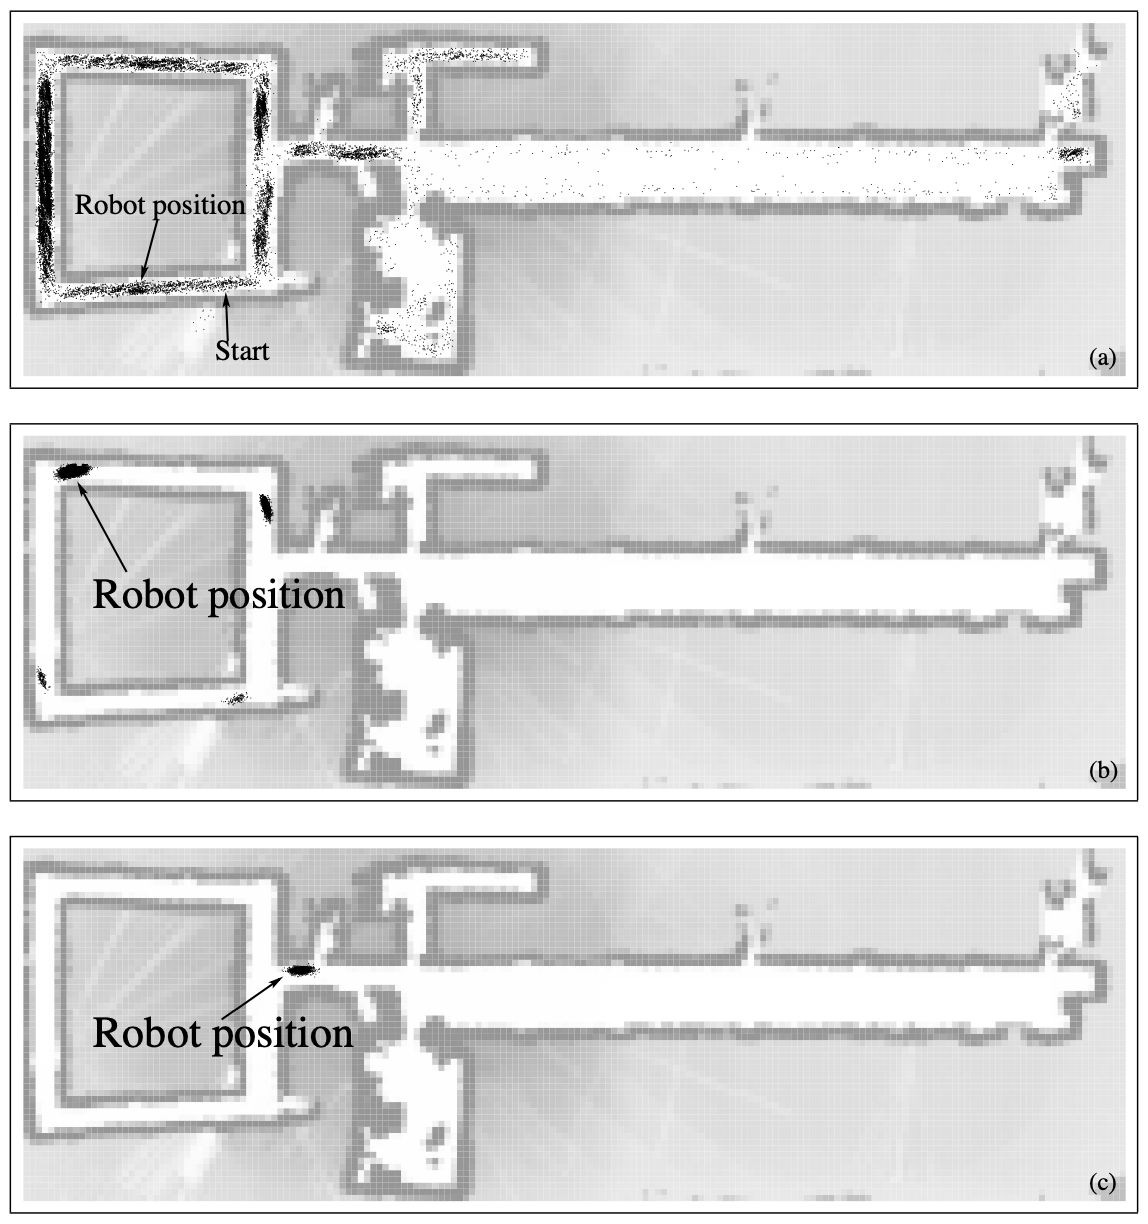
\includegraphics[width=8cm]{AMCL}
    \centering
    \caption{Change in the probability distribution of a robot's position (belief) with time \parencite{thrunProbabilisticRobotics2006}. In Adaptive Monte Carlo Localization (AMCL), this distribution is approximated by a set of particles, each representing a possible robot pose. While each particle also has an associated direction, it's omitted from the figure due to clutter.}
    \label{fig:belief}
\end{figure}

\todo{May need some work}